\section{Results}
\label{sec:results}

\subsection{Faster matrix multiplication via finding novel algorithms for tensor decomposition}
\label{subsec:matmul}

\begin{table}[t]
\rowcolors{2}{white}{lightgray}
\begin{center}
    \begin{tabular}{ccc}
    $\langle m, n, p \rangle$ & best known [reference] & \method \\ \midrule
    $\langle 2, 4, 5 \rangle$ & 33 \citep{hopcroft} & \textbf{32} \\
    $\langle 2, 4, 7 \rangle$ & 46 \citep{smirnov2013bilinear} & \textbf{45} \\
    $\langle 2, 4, 8 \rangle$ & 52 \citep{smirnov2013bilinear} & \textbf{51} \\
    $\langle 2, 5, 6 \rangle$ & 48 \citep{smirnov2013bilinear}   & \textbf{47}    \\ 
    $\langle 3, 3, 3 \rangle$ & 23 \citep{laderman}   & 23   \\
    $\langle 3, 4, 6 \rangle$ & 56 \citep{Kauers_2025}   & \textbf{54}   \\ 
    $\langle 3, 4, 7 \rangle$ & 66 \citep{smirnov2021}   & \textbf{63}   \\ 
    $\langle 3, 4, 8 \rangle$ & 75 \citep{smirnov2021}   & \textbf{74}    \\ 
    $\langle 3, 5, 6 \rangle$ & 70 \citep{Kauers_2025}   & \textbf{68}    \\
    $\langle 3, 5, 7 \rangle$ & 82 \citep{smirnov2021}   & \textbf{80}    \\ 
    $\langle 4, 4, 4 \rangle$ & 49 \citep{strassen1969gaussian}   & \textbf{48}  \\ 
    $\langle 4, 4, 5 \rangle$ & 62 \citep{kauers2023flip}   & \textbf{61}    \\
    $\langle 4, 4, 7 \rangle$ & 87 \citep{smirnov2013bilinear} & \textbf{85}    \\
    $\langle 4, 4, 8 \rangle$ & 98~\citep{strassen1969gaussian} & {\textbf{96}} \\ 
    $\langle 4, 5, 6 \rangle$ & 93 \citep{Kauers_2025}   & \textbf{90}    \\ 
    $\langle 5, 5, 5 \rangle$ & 93 \citep{flip_graphs_with_symmetry}  & 93  \\ 
    \end{tabular}
\caption{%
Upper bounds on the rank of the tensor $\langle m,n,p \rangle$ representing the product of an $m\times n$ matrix and an $n\times p$ matrix, i.e.~the number of scalar multiplications required to compute this matrix product.
Beyond the examples shown here, for all parameters $m,n,p\leq 5$, \method either matched or surpassed the best known solutions, and provided exact algorithms (see \Cref{tab:relaxed-opt-results-appendix} in appendix for full results).
For $\langle 3, 4, 7\rangle$, $\langle 4, 4, 4\rangle$, and $\langle 4, 4, 8\rangle$, the algorithms discovered by \method use complex-valued multiplications which can be used for exact multiplication of complex or real-valued matrices.
The decompositions shown in this table can be found in \ResultsColab.%
}
    \label{tab:relaxed-opt-results}
\end{center}
\end{table}

From accelerating machine learning computations to enabling realistic computer graphics, matrix multiplication serves as a fundamental operation underpinning numerous critical algorithms and applications within computer science.
Since the pioneering work of \citet{strassen1969gaussian}, it has been known that a rich space of algorithms for multiplying two matrices can be represented as decompositions of a given 3D tensor into rank-one tensors.
The rank (number of terms) of the decomposition exactly specifies the number of scalar multiplications needed to compute the matrix product.
Hence, to develop faster matrix multiplication algorithms one needs to find low-rank decompositions of particular tensors.
This problem has been tackled with many approaches, from specialized alternating least squares solvers~\citep{smirnov2013bilinear} to deep reinforcement learning~\citep{fawzi2022discovering} and custom search algorithms~\cite{kauers2023flip}; yet, despite decades of effort, even for the simple case of multiplying two $3\times 3$ matrices, the minimum achievable rank is not known, showcasing the difficulty of the problem.

Starting from the problem description and a standard gradient-based algorithm (including an initializer, a reconstruction loss function, and an Adam optimizer~\cite{kingma2015adam}), \method is able to develop sophisticated tensor decomposition algorithms that outperform existing approaches.
To evaluate each evolved program, we choose a set of matrix multiplication targets and run the algorithm, initialized with multiple random seeds using the evaluation cascade described in \Cref{subsec:evaluation}. 
The performance is then measured as the best (lowest) rank achieved on each target as well as the fraction of seeds that achieved this rank, providing a signal for \method to hill-climb.
To ensure the exactness of the decomposition and avoid any potential numerical error, when evaluating, we round each element to the nearest integer or the nearest half-integer; and, to encourage the algorithm to generate near-integral solutions, we include this request in natural language in the LLM's prompt.

\begin{figure}[p]
\vspace{-0.03\textwidth}
\hspace{-0.1\textwidth}
\begin{minipage}{0.32\textwidth}
% Does not work in newer versions of pdflatex -- runs out of memory.
%\lstinputlisting[style=pydiffsmall, backgroundcolor=\color{backcolour}]{code/diff_full.diff}
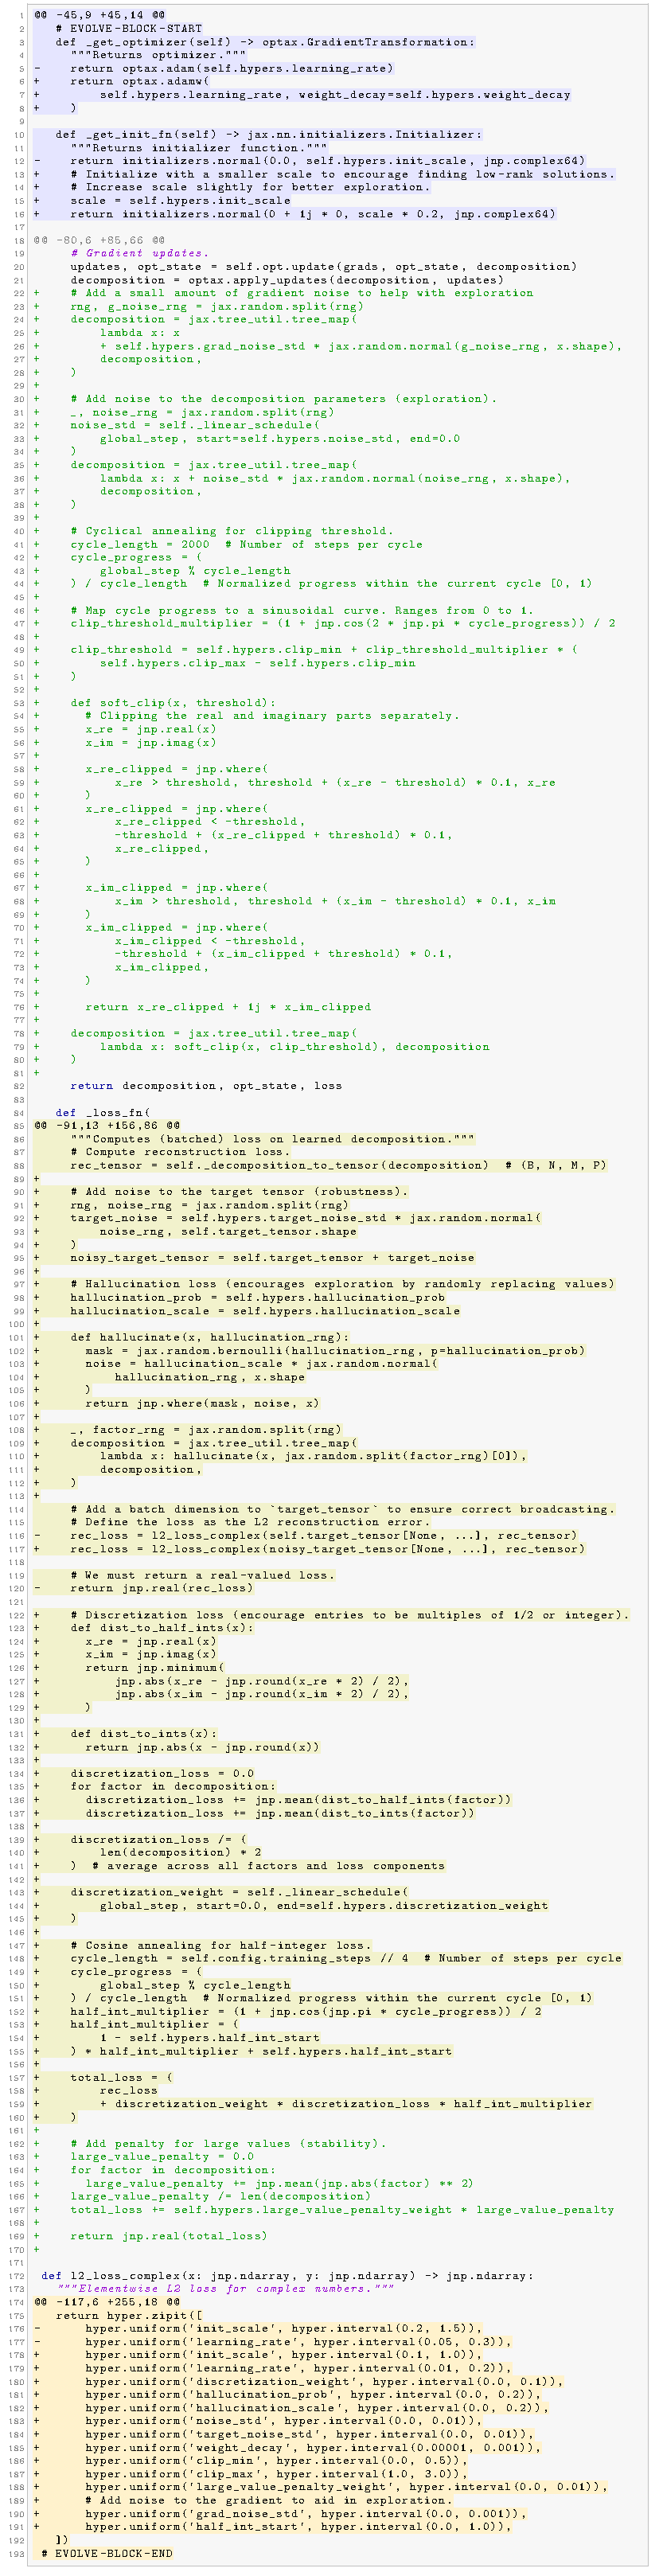
\includegraphics[width=\linewidth]{code/diff_full.pdf}
\end{minipage}
\hspace{0.06\textwidth}
\begin{minipage}{0.59\textwidth}%
\lstinputlisting[style=pydiffmedium, backgroundcolor=\color{highlightblue}]{code/zoom1.diff}
\vspace{-0.4em}
\lstinputlisting[style=pydiffmedium, backgroundcolor=\color{highlightyellow}]{code/zoom2.diff}
\vspace{-0.4em}
\lstinputlisting[style=pydiffmedium, backgroundcolor=\color{highlightorange}]{code/zoom3.diff}
\end{minipage}
\hspace{-0.1\textwidth}
\caption{Changes proposed by \method to discover faster matrix multiplication algorithms. The full diff is outlined on the left (see magnified version in~\Cref{fig:relaxed-opt-diff-appendix-1,fig:relaxed-opt-diff-appendix-2,fig:relaxed-opt-diff-appendix-3}) and some excerpts are highlighted on the right. In this example, \method proposes extensive changes across several components, including the optimizer and weight initialization (top right), the loss function (middle right), and hyperparameter sweep (bottom right). These changes are highly non-trivial, requiring 15 mutations during the evolutionary process.}\label{fig:relaxed-opt-diff}
\centering
\end{figure}


In Table~\ref{tab:relaxed-opt-results}, one can see that the various algorithms developed by \method improve the state of the art for 14 different matrix multiplication targets.
Notably, for multiplying two $4\times 4$ matrices, applying the algorithm of \citet{strassen1969gaussian} recursively results in an algorithm with rank (number of scalar multiplications) equal to 49, which works over any field.
For the very specific case of multiplying in the field with 2 elements,~\citet{fawzi2022discovering} found an algorithm with rank 47.
For 56 years, designing an algorithm with rank less than 49 over any field with characteristic 0 was an open problem.%
\footnote{There exist algorithms using fewer than 49 multiplications, but they do not correspond to decompositions of the matrix multiplication tensor, and they cannot be applied recursively to multiplying larger matrices.\vspace{-1em}}
\method is the first method to find a rank-$48$ algorithm to multiply two $4\times 4$ complex-valued matrices.

As shown in Figure~\ref{fig:relaxed-opt-diff}, \method makes significant changes to the initial program, introducing several original ideas to design increasingly better algorithms.
While most results in Table~\ref{tab:relaxed-opt-results} (including $\langle 4, 4, 4 \rangle$) were obtained from a simple initial program, we found that for some parameters, seeding the initial program with our own ideas (such as adding stochasticity to the evaluation function or using evolutionary approaches) could further boost performance, highlighting the possibility of scientific collaboration between researchers and \method. 


\subsection{Finding tailored search algorithms for a wide range of open mathematical problems}
\label{subsec:math}

A significant frontier in mathematical research involves discovering objects or \textit{constructions} that possess optimal, or near-optimal, properties according to some measure. Examples range from finding dense packings of geometric shapes~\cite{geometry_collection} to identifying functions or sets satisfying specific combinatorial or analytic constraints~(e.g., \cite{matolcsi2010improved, vinuesa2010generalized, haugland2016minimum, gyarmati2007sums}). Progress often relies on finding a single construction that surpasses all previously known examples, thereby establishing new lower or upper bounds for the optimal value. We demonstrate that \method serves as a powerful tool for exploring the vast search space inherent in these problems, successfully tackling a diverse array of open mathematical challenges.

To assess its capabilities, we apply \method to a curated set of over 50 mathematical problems, spanning more than five different branches of mathematics, including analysis, combinatorics, number theory, and geometry, evaluated across numerous specific parameter settings (e.g., different dimensions or sizes). In 75\% of the cases \method rediscovered the best known constructions, and in 20\% of the cases it discovered a new object that is better than a previously known best construction, thereby improving the SOTA. In all these cases, the initial starting point was a simple or a random construction. These results underscore \method's broad potential as a versatile tool for mathematical research.

\begin{figure}[t]
    \centering
    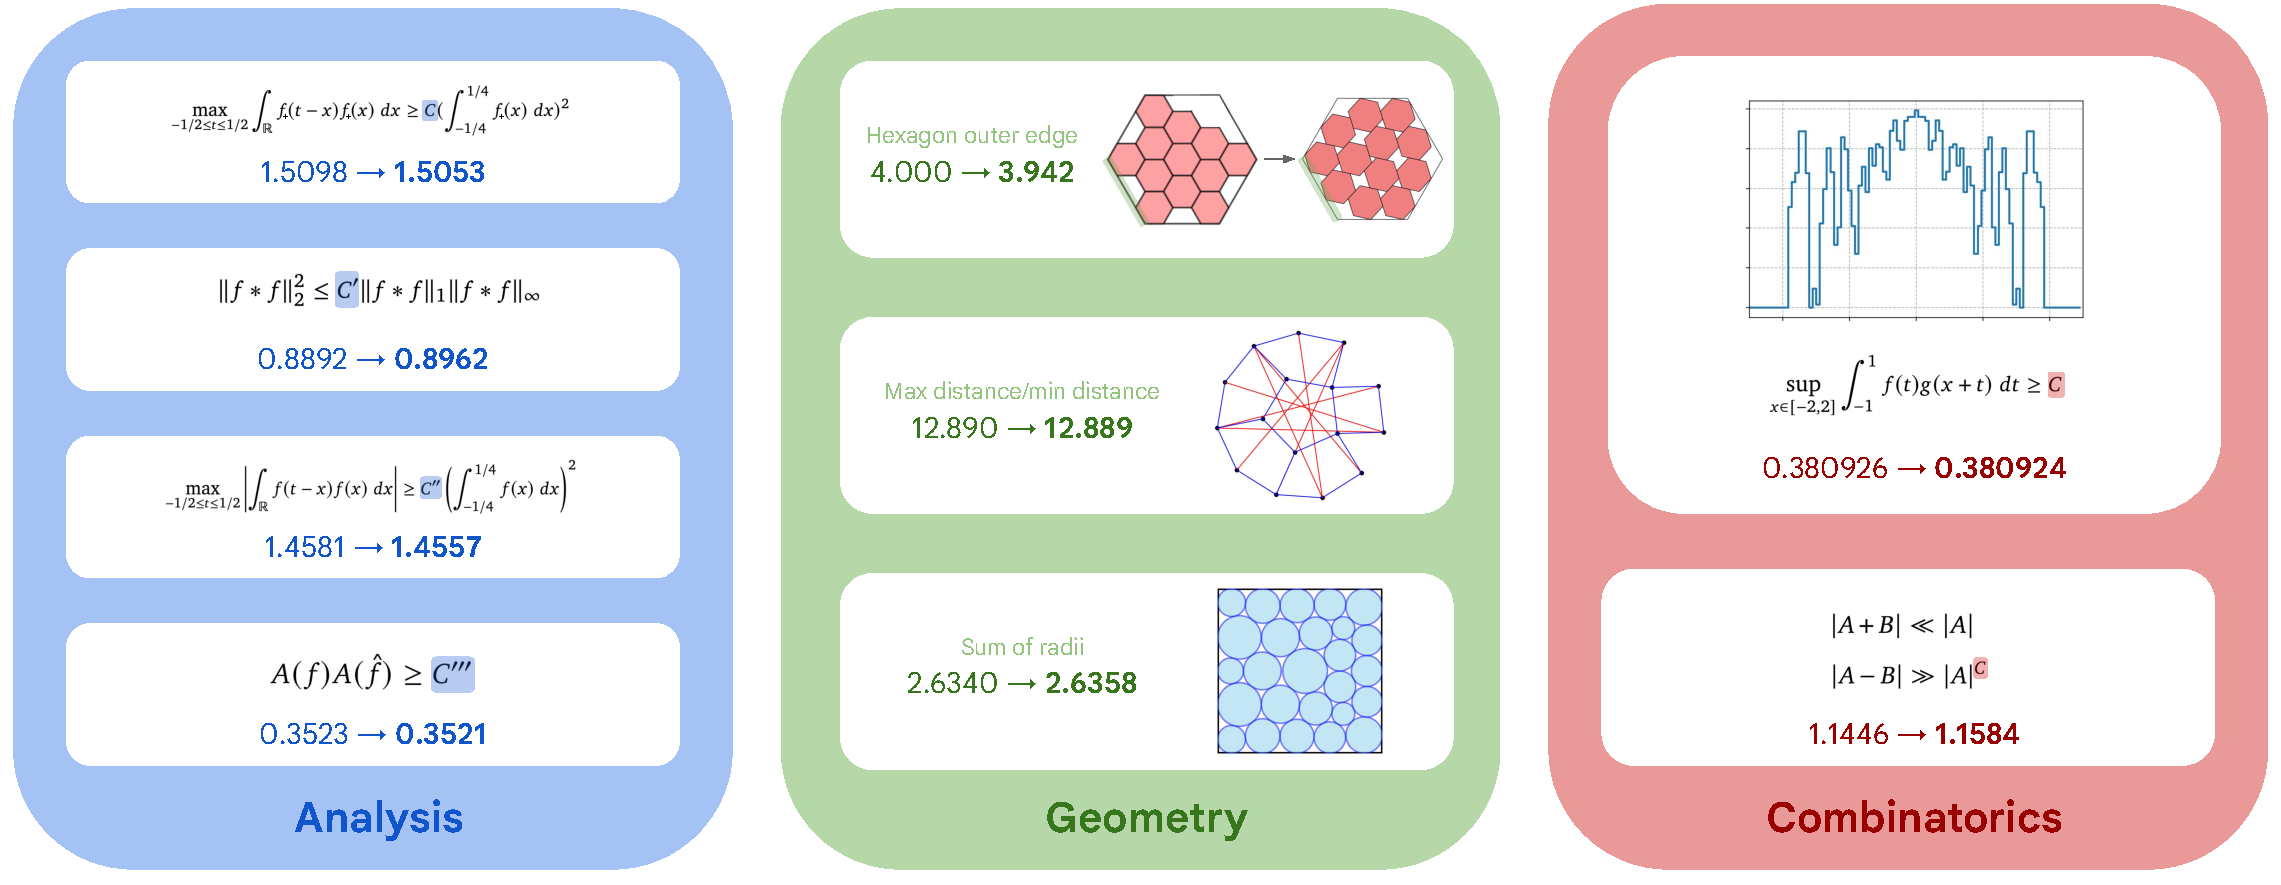
\includegraphics[width=1.0\textwidth]{figures/math_results.pdf}
    \caption{Examples of SOTA-breaking mathematical constructions discovered with \method. The versatility of \method allows us to tackle problems in analysis (autocorrelation and uncertainty inequalities), geometry (packing and minimum/maximum distance problems) and combinatorics (Erd\H{o}s's minimum overlap problem and sums and differences of finite sets).}
    \label{fig:math_sota_examples}
\end{figure}

\newpage % to avoid splitting the paragraph into 3 pages.
A significant advantage of the \method configuration used here is its versatility and speed of application. The core methodology, focused on evolving heuristic search programs (detailed below), can be rapidly deployed across a diverse range of mathematical construction problems and conjectures, often requiring less initial problem-specific expert tailoring compared to traditional bespoke approaches. While deep mathematical insight naturally aids in problem formulation and search space definition, \method often demonstrates a capacity to autonomously discover effective search patterns and attack strategies by identifying subtle structures within the problem landscape. This allows for efficient, large-scale exploration across many different problems.

The key methodological innovation enabling these discoveries is \method's ability to evolve \textit{heuristic search algorithms} rather than directly evolving the constructions themselves. For many problems, particularly those with fast objective function evaluations---which are common in mathematics---we employed an iterative refinement strategy. Each generation of \method was tasked with evolving a program representing a search heuristic. This program was given a fixed time budget (e.g., 1000 seconds) and was shown the best construction found by the previous best heuristic. Its goal was to leverage this starting point and the allotted time to find an even better construction. The evolutionary process thus selects for heuristics that are effective at improving already high-quality solutions. The final constructions were often the result of a sequence of different, specialized heuristics discovered by \method---early heuristics proficient at making large gains from random or simple initial states, and later heuristics adept at fine-tuning near-optimal configurations. This automated discovery of multi-stage, adaptive search strategies is challenging to replicate manually and proved crucial for surpassing the SOTA.

Below are high-level descriptions of some of the problems where \method yielded new results. Full list of problems and details are provided in Appendix~\ref{app:maths}.

\begin{itemize}
    \item \textbf{Analysis} 
    \begin{itemize}
        \item \textbf{Autocorrelation inequalities.} \method was able to improve the best known bounds on several autocorrelation inequalities.
        \item \textbf{Uncertainty principles.} \method was able to produce a refined configuration for a problem arising in Fourier analysis, by polishing an uncertainty principle construction \cite{gonccalves2017hermite} leading to a slightly better upper bound. 
    \end{itemize}

    \item \textbf{Combinatorics and number theory}
        \begin{itemize}
            \item \textbf{Erd\H{o}s's minimum overlap problem.} \method established a new upper bound for the minimum overlap problem~\cite{erdHos1955some}, slightly improving upon the previous record~\cite{haugland2016minimum}.
        \end{itemize}

    \item \textbf{Geometry and packing}
        \begin{itemize}
            \item \textbf{Kissing number problem.} In 11 dimensions, \method improved the lower bound on the kissing number, finding a configuration of 593 non-overlapping unit spheres that can simultaneously touch a central unit sphere, surpassing the previous record of 592~\citep{kissing_11}. 
            \item \textbf{Packing problems.} \method achieved several new results in packing problems, such as packing $N$ points in a shape to minimize the ratio of the maximum and minimum distance, packing various polygons in other polygons in the most efficient way, and variants of the Heilbronn problem concerning point sets avoiding small-area triangles~\cite{geometry_collection}.
        \end{itemize}
\end{itemize}

The full list of problems appears in Appendix~\ref{app:maths} and the new constructions found by \method can be found in~\ResultsColab.
More examples and details on these problems and the methods used will be provided in an upcoming paper.
Most of these discoveries are on open problems suggested to us by external mathematicians Javier Gomez Serrano and Terence Tao, who also advised on how to best formulate them as inputs to \method.
This highlights the potential for synergistic partnerships between AI-driven discovery engines like \method and human mathematical expertise.


\subsection{Optimizing Google's computing ecosystem}

In addition to the scientific applications presented in preceding sections, here we demonstrate how \method has been used to improve performance of mission-critical infrastructure and deliver real-world impact.

\subsubsection{Improving data center scheduling}

Efficiently scheduling compute jobs onto a cluster of machines is a critical optimization problem, particularly at the scale of Google's data centers, orchestrated by Borg \cite{43438}. This task involves assigning jobs to available machines based on job resource requirements and machine capacity. Inefficient assignments can result in stranded resources: when a machine can no longer accept jobs because it has run out of one kind of resource (e.g., memory) but still has other resources free (e.g., CPU). Improvements in scheduling efficiency can recover these stranded resources, allowing more jobs to be completed on the same amount of computational footprint. This recovery is essential to accommodate growing compute needs without a proportional increase in resource consumption. Furthermore, this problem is challenging since it combines typical engineering difficulties, such as debuggability and scale, on top of the classically difficult bin-packing problem.

We address this challenge by framing the online job scheduling problem as a vector bin-packing problem with two variables. In this context, machines represent bins with defined capacities for CPU and memory, and incoming jobs are items with specific resource demands. A heuristic function takes as input a pending job’s CPU and memory requirements and a potential machine’s CPU and memory availability. This function then outputs a priority score for the machine. The Borg scheduler subsequently assigns the pending job to the machine with the highest priority score as determined by the heuristic function, among other objectives. Because this heuristic only influences the ranking of machines already determined by Borg to be available and capable of running each pending job, the resulting scheduling decisions are effectively correct by construction.

An early version of \method was used to discover a remarkably simple yet effective heuristic function (shown in \Cref{fig:alphaevolve_heuristic}), evolving from the existing one in production. We use a simulator of our data centers to provide feedback to \method based on historical snapshots of workloads and capacity across Google’s fleet. We measure the performance of \method's heuristic function on an unseen test dataset of recent workloads and capacity to ensure generalization. Observing that \method's heuristic function outperforms the one in production, we rolled out \method's heuristic function to the entire fleet. Post-deployment measurements across Google’s fleet confirmed the simulator results, revealing that this heuristic function continuously recovers on average 0.7\% of Google’s fleet-wide compute resources, which would otherwise be stranded. \method was chosen over a deep reinforcement learning approach because its code solution not only leads to better performance, but also offers clear advantages in interpretability, debuggability, predictability, and ease of deployment—essential qualities for a mission-critical system.

\begin{figure}[t]
\centering

\begin{minipage}[c]{0.55\textwidth}
\centering
\begin{minted}[
    linenos,
    breaklines=false,]{python}
def alpha_evolve_score(required, free):
  cpu_residual = required.cpu / free.cpu
  mem_residual = required.mem / free.mem

  return -1.0 * (cpu_residual + mem_residual +
                 mem_residual / cpu_residual +
                 cpu_residual / mem_residual)
\end{minted}
\end{minipage}
\hfill
\begin{minipage}[c]{0.4\textwidth}
    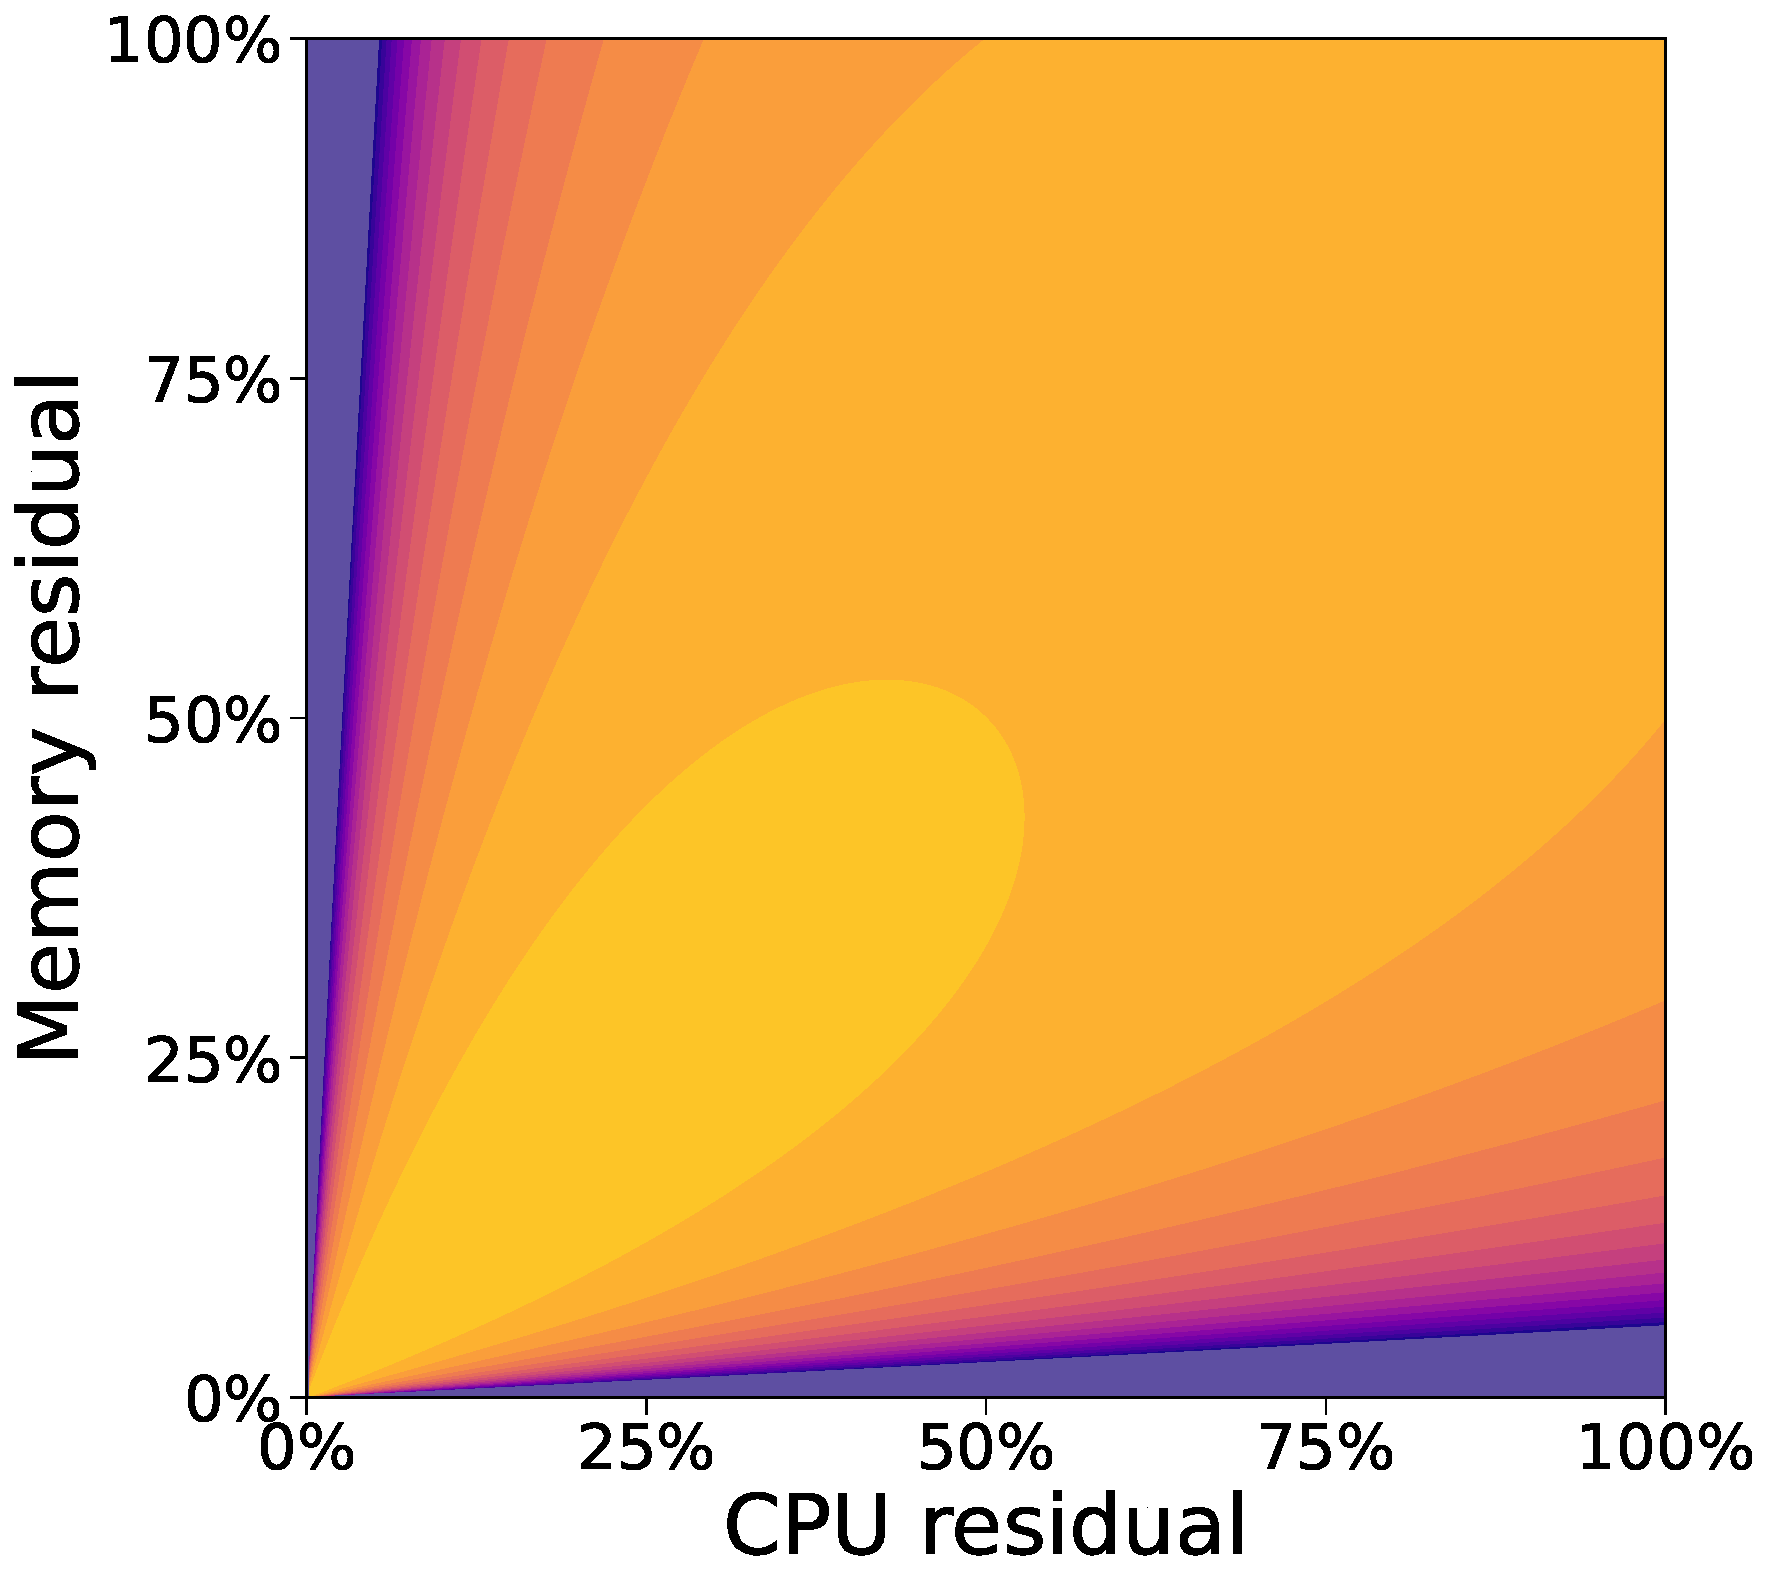
\includegraphics[width=1.0\textwidth]{figures/borg_heuristic.pdf}
\end{minipage}

\caption{Left: The heuristic function discovered by \method, tailored to Google’s workloads and capacity. Right: Visualization of the heuristic scoring function. Yellow regions represent high scores, while purple regions represent low scores.}
\label{fig:alphaevolve_heuristic}
\end{figure}


\subsubsection{Enhancing Gemini kernel engineering}

Training large models like Gemini requires substantial computational resources. Gemini is built on JAX \cite{jax2018github}, and Pallas is an extension to JAX that enables writing custom, highly specialized programs (kernels) tailored for optimal execution on hardware accelerators. Therefore, efficient Pallas kernels are crucial for optimizing Gemini’s training performance. A critical aspect of kernel optimization is tuning the tiling strategy for matrix multiplication operations (see~\Cref{fig:tiling_heuristic}). This technique involves dividing a large matrix multiplication computation into smaller subproblems to better balance computation with data movement, which is key to accelerating the overall computation. Traditionally, kernel engineers rely on either search-based autotuning or manually crafted heuristics to determine near-optimal tiling configurations for various input shapes. Search-based tuning interrupts the research workflow, necessitating retuning for every input shape change. Conversely, manually crafting effective tiling heuristics is a major engineering bottleneck due to its complexity, demanding a deep understanding of both kernel functionality and hardware intricacies. The key advantage of a performant heuristic is its ability to deliver high performance across arbitrary input shapes. Consequently, to expedite the design of performant kernels for emerging hardware and to simplify their utilization by model developers, we aim to facilitate the heuristic generation process.

\begin{figure}[t]
    \centering
    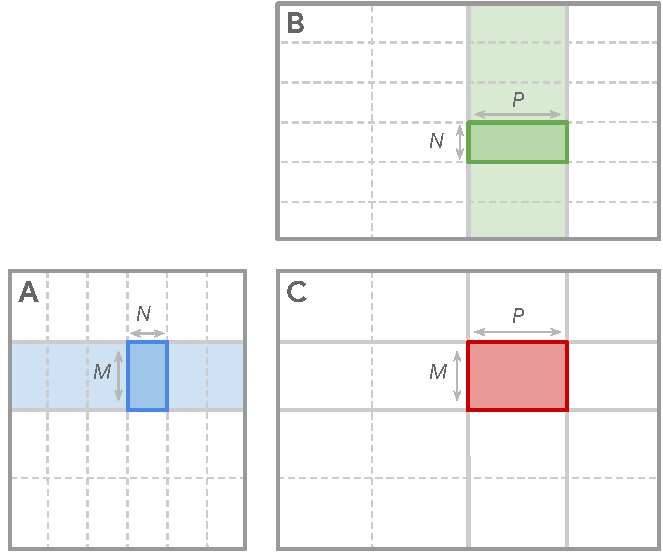
\includegraphics[width=0.5\textwidth]{figures/matmul_tiling_figure.pdf}
    \caption{Visualization of the tiling heuristic problem for a matrix  product $AB = C$. Creating a heuristic that automatically chooses the right tile size ($M$, $N$, $P$) for all input shapes is difficult because one has to know the matrix multiplication unit’s optimal shapes and memory capacity, the memory requirements of surrounding operations, extra operations that are fused into the kernel, and low-level compiler intricacies, among other details.}
    \label{fig:tiling_heuristic}
\end{figure}

We address this challenge by employing \method to optimize tiling heuristics for an important matrix multiplication kernel used to train Gemini. The objective is to minimize the kernel's actual runtime. \method iteratively explores and refines tiling heuristics for this kernel by proposing candidate code, aiming to minimize this runtime on various input shapes on real TPU accelerators. The kernel’s correctness is maintained by construction because \method is optimizing the tiling strategy for this kernel rather than altering its underlying mathematical operation. To build the training and evaluation datasets for \method, we automatically collect realistic kernel input shapes from kernel users. Half of these input shapes form the training set, providing the optimization targets during the evolutionary process. The remaining input shapes form the evaluation set, used to test the general applicability of the resulting heuristic.

This automated approach enables \method to discover a heuristic that yields an average 23\% kernel speedup across all kernels over the existing expert-designed heuristic, and a corresponding 1\% reduction in Gemini’s overall training time. In addition, the use of \method significantly reduced the kernel optimization time, from several months of dedicated engineering effort to just days of automated experimentation. This acceleration speeds up the deployment of optimized kernels, allowing kernel engineers to dedicate their expertise to more strategic, higher-level optimization problems. Furthermore, \method offers a path towards automating the manual tuning process and improving the ergonomics of Gemini kernel usage. The tiling heuristic discovered by \method has been deployed in production, directly enhancing Gemini's training efficiency and the Gemini team’s research and engineering velocity. This deployment also marks a novel instance where Gemini, through the capabilities of \method, optimizes its own training process.


\subsubsection{Assisting in hardware circuit design}

Specialized hardware, such as Google's Tensor Processing Units (TPUs), is crucial for achieving the resource efficiency required to run modern AI systems at scale. However, designing new computer chips is a complex and time-consuming process, often spanning years. Register-Transfer Level (RTL) optimization, a critical step in this process, involves manually rewriting hardware descriptions to improve metrics like power, performance, and area, demanding months of iteration by highly skilled engineers.

In this work, \method was challenged to optimize an already highly optimized Verilog implementation of a key TPU arithmetic circuit within the matrix multiplication unit. The optimization objectives were to reduce both area and power consumption while preserving the component's core functionality. Crucially, the final proposal must pass robust verification methods to confirm that the modified circuit maintains functional correctness. \method was able to find a simple code rewrite that removed unnecessary bits, a change validated by TPU designers for correctness. While this specific improvement was also independently caught by downstream synthesis tools, \method's contribution at the RTL stage demonstrates its capability to refine source RTL and provide optimizations early in the design flow.

Integrated into an upcoming TPU, this improvement represents Gemini’s first direct contribution to TPU arithmetic circuits, achieved via \method, paving the way for future contributions. A key advantage of \method is that it communicates the suggested changes directly in Verilog, the standard language used by hardware engineers, fostering trust and simplifying adoption. This early exploration demonstrates a novel approach where LLM-powered code evolution assists in hardware design, potentially reducing time to market.


\subsubsection{Directly optimizing compiler-generated code}

The transformer architecture~\cite{vaswani2017attention} is used in the majority of modern neural networks, ranging from LLMs to AlphaFold~\cite{alphafold3}. 
The core computation of transformers is the attention mechanism~\cite{bahdanau2014neural}, which is most commonly implemented using FlashAttention~\cite{dao2022flashattention}.
In our stack, FlashAttention is implemented as an accelerator kernel in Pallas, wrapped by higher-level code in JAX that handles input preparation and output postprocessing.
The machine learning compiler (XLA~\cite{xla}) then translates this implementation into a sequence of intermediate representations (IRs), each adding more detail for execution on particular hardware. At these stages, improved decisions on memory access orchestration or computation scheduling can significantly reduce runtime on specific hardware.

We challenged \method to directly optimize the XLA-generated IRs encapsulating the FlashAttention kernel along with pre- and postprocessing code. We optimized a configuration corresponding to a highly impactful transformer model used for inference at scale on GPUs, with the goal of minimizing the module's overall execution time. This was a particularly challenging task, because (1) the IR is designed for debugging purposes rather than for direct editing by developers, and (2) it is compiler-generated and already highly optimized. Each modification proposed by \method was checked against the reference (unmodified) code on randomized inputs in order to ensure numerical correctness throughout optimization. The final version of the code was rigorously confirmed by human experts to be correct for all possible inputs.

\method was able to provide meaningful optimizations for both levels of abstraction exposed by the IR. Firstly, the FlashAttention kernel for the configuration of interest was sped up by 32\%. Secondly, \method found improvements in pre- and postprocessing of kernel inputs and outputs, resulting in a 15\% speed up in this part. These results demonstrate the ability of \method to optimize compiler-generated code, offering the potential of incorporating discovered optimizations into existing compilers for specific use cases, or, in the longer term, incorporating \method into the compiler workflow itself.
